\chapter{Dasar Teori}
\label{chap:dasarteori}

\section{\textit{Mobile Cloud Computing}}
\label{sec:mobilecloudcomputing}

\section{Android}
\label{sec:android}

Pada sub-bab ini akan dibahas mengenai pengertian dan arsitektur Android.

\subsection{Pengertian Android}
\label{subsec:pengertianandroid}

Android merupakan sistem operasi untuk \textit{mobile device}.

\subsection{Arsitektur Android}
\label{subsec:arsitektur}

Secara umum arsitektur Android dibagi menjadi empat lapisan dapat dilihat pada Gambar~\ref{fig:arsitektur_android}, yaitu\footnote{http://elinux.org/Android\_Architecture}:

\begin{enumerate}
\item \textit{Applications} merupakan lapisan teratas yang berhubungan dengan para pengguna.
\item \textit{Applications Framework} merupakan lapisan yang diperuntungkan kepada para penggembang aplikasi. Pada lapisan ini terdapat \textit{framework} yang dapat digunakan orang para pengembang aplikasi.
\item \textit{Libraries} merupakan kumpulan-kumpulan fungsi yang disediakan oleh Android.
\item \textit{Linux Kernel} merupakan kumpulan-kumpulan fungsi yang berhubungan langsung dengan perangkat keras.
\end{enumerate}

\begin{figure}
\centering
\resizebox{\textwidth}{!}{
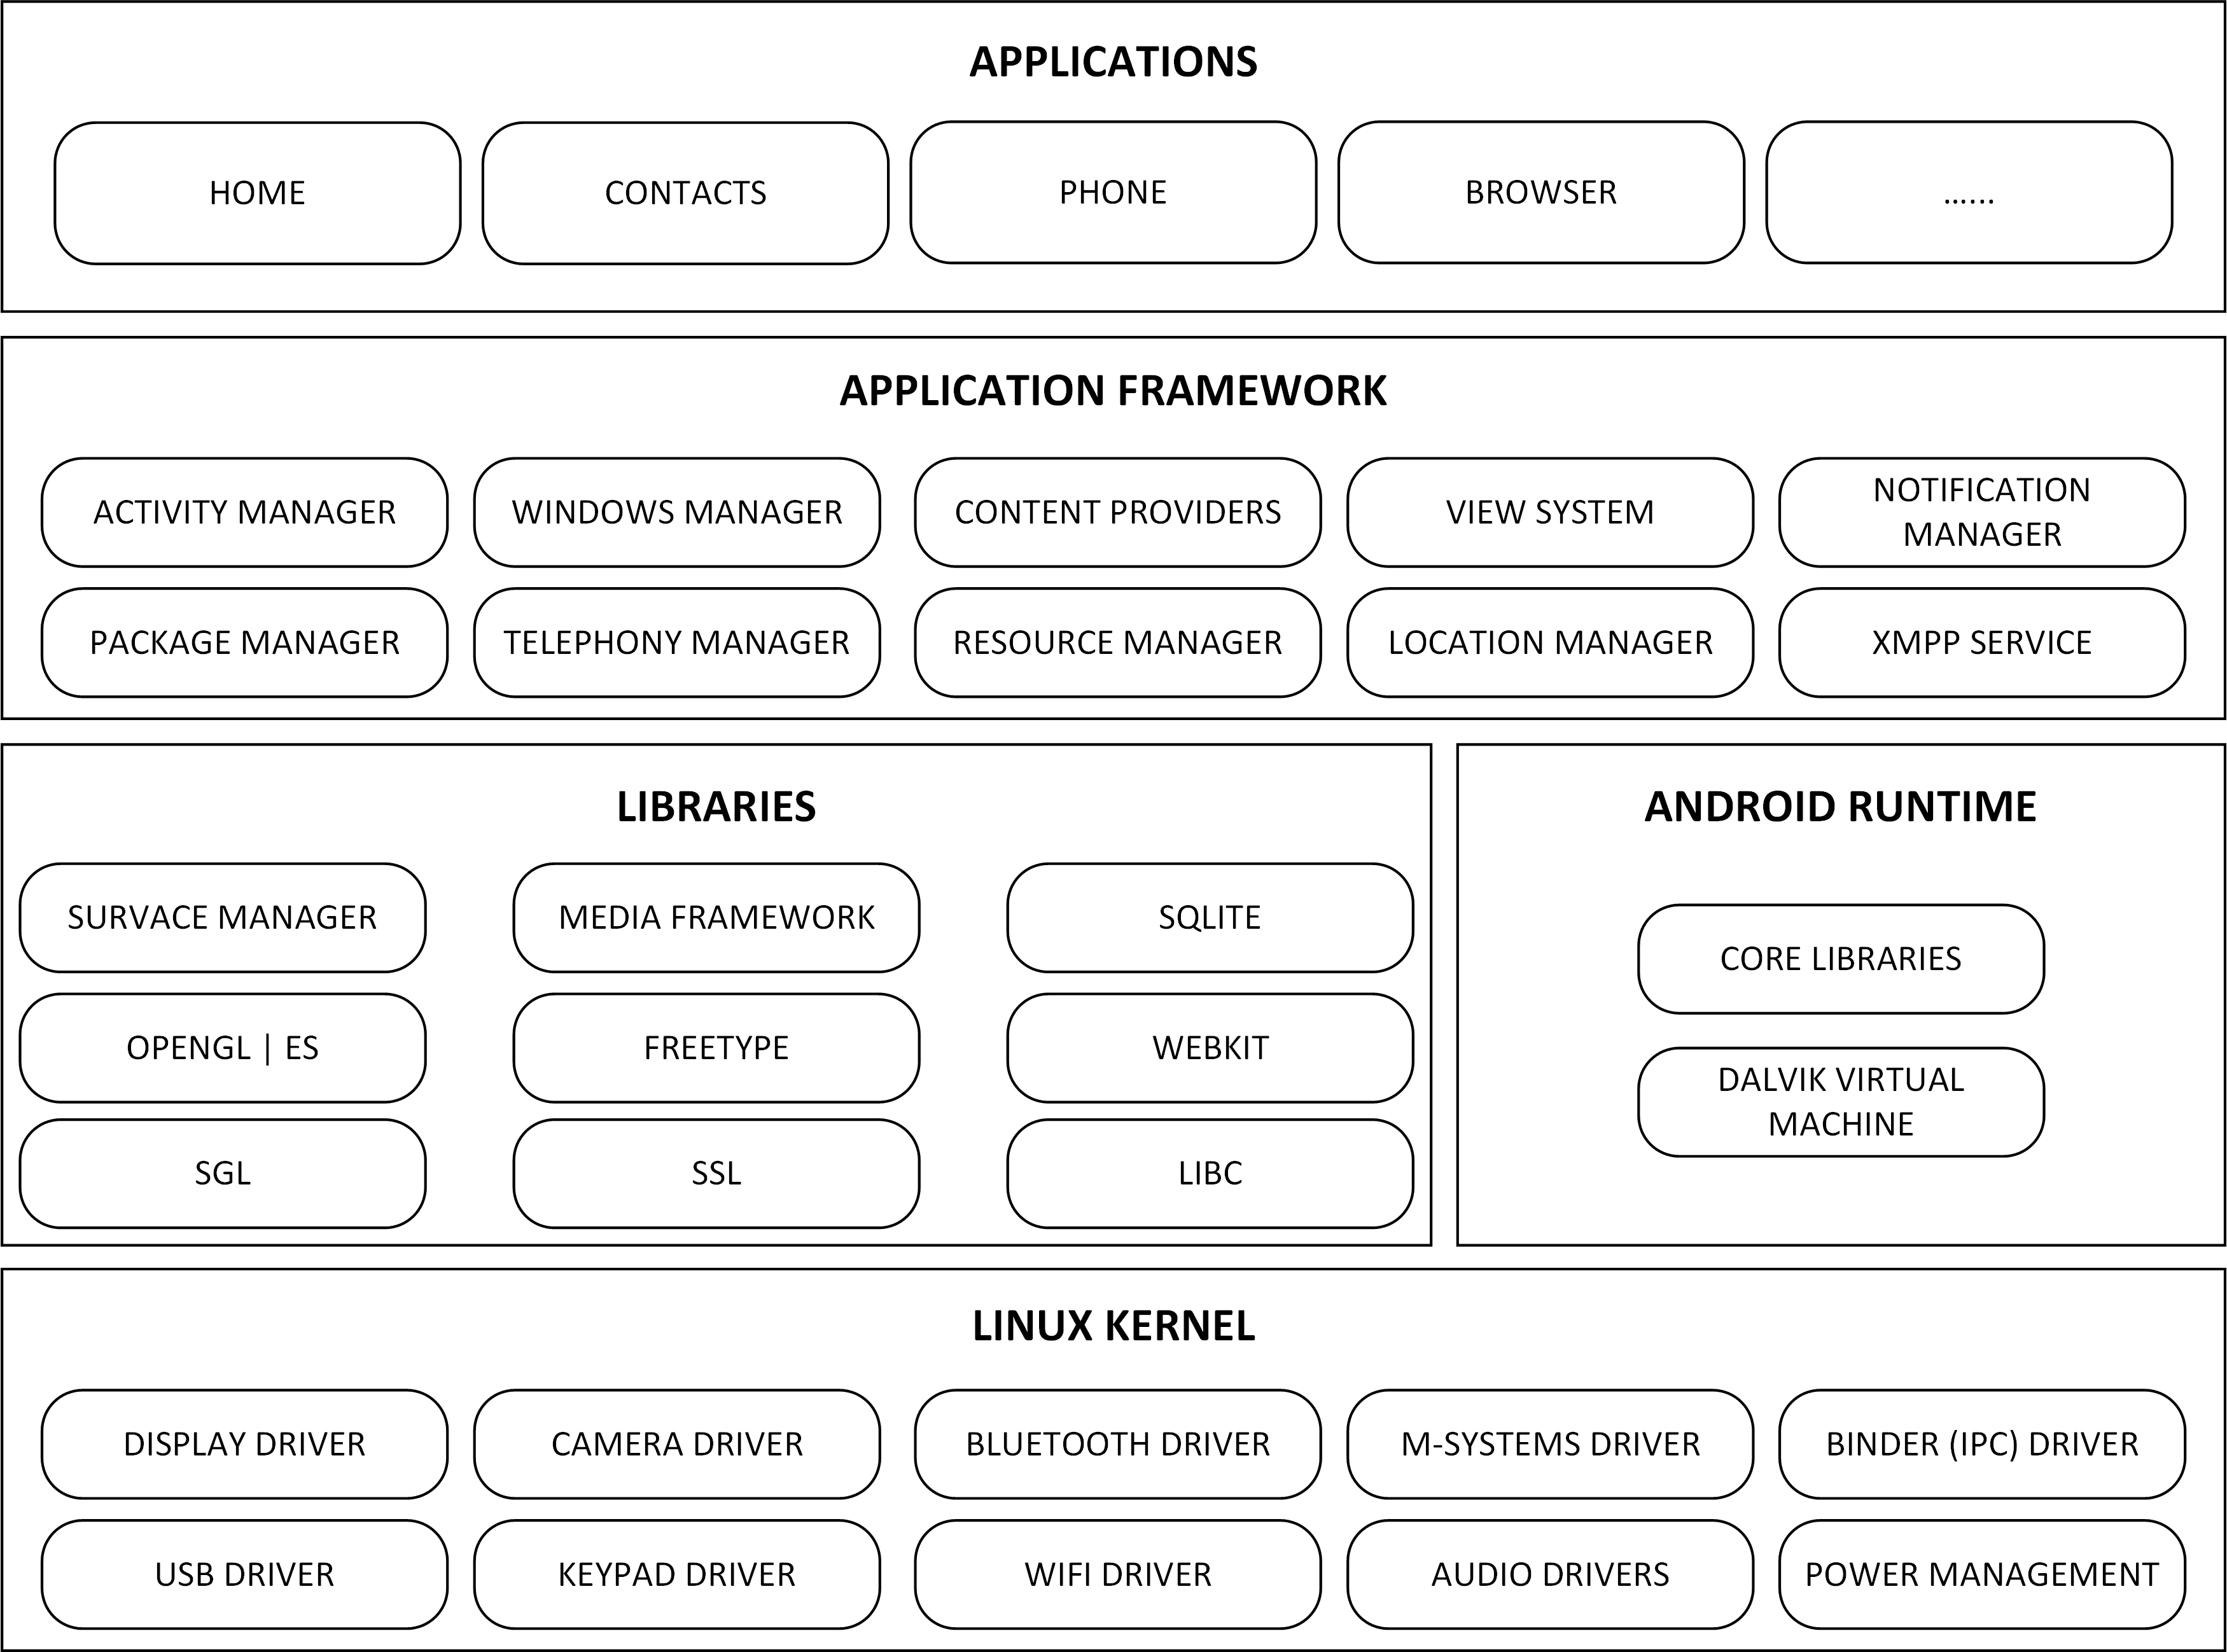
\includegraphics{Gambar/Android-system-architecture}
}
\caption[Arsitektur Android]{Arsitektur Android} 
\label{fig:arsitektur_android}
\end{figure}

\subsection{\textit{Life Cycle}}
\label{subsec:lifecycle}

Aplikasi yang berjalan di Android memiliki \textit{lifecycle} sesuai dengan  rancangan sistem operasi tersebut dapat dilihat pada gambar \ref{fig:dasar_lifecycle_android}.

\begin{figure}
\centering
\resizebox{\textwidth}{!}{
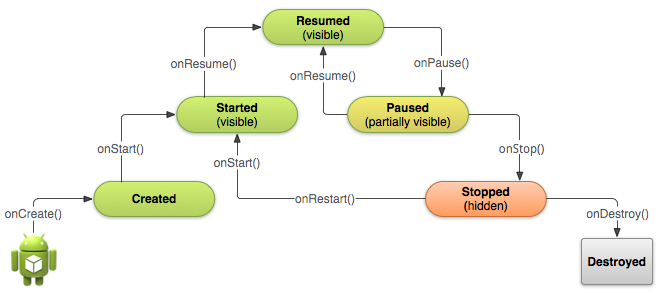
\includegraphics{Gambar/basic-lifecycle}
}
\caption[Dasar \textit{lifecycle} Android]{Dasar \textit{lifecycle} Android} 
\label{fig:dasar_lifecycle_android}
\end{figure}

\section{Phonegap}
\label{sec:phonegap}

\subsection{Pengertian Phonegap}
\label{sec:pengertianphonegap}

Phonegap merupakan suatu framework untuk mengembangkan aplikasi pada \text{device mobile}. Phonegap memungkinkan aplikasi dibangun di atas Javascript, HTML5, dan CSS3\footnote{Jose Fermoso (April 5, 2009). "PhoneGap Seeks to Bridge the Gap Between Mobile App Platforms"}.

\subsection{Arsitektur Phonegap}
\label{sec:arsitekturphoengap}

Phonegap menggunakan HTML5 dan CSS3 untuk men-\textit{render} aplikasi dan Javascript untuk logikanya. Phonegap membangun API yang dapat digunakan oleh pengembang aplikasi di atas OS \textit{mobile device}. Arsitektur Phonegap dapat dilihat pada Gambar~\ref{fig:arsitektur_phonegap} 

\begin{figure}
\centering
\resizebox{\textwidth}{!}{
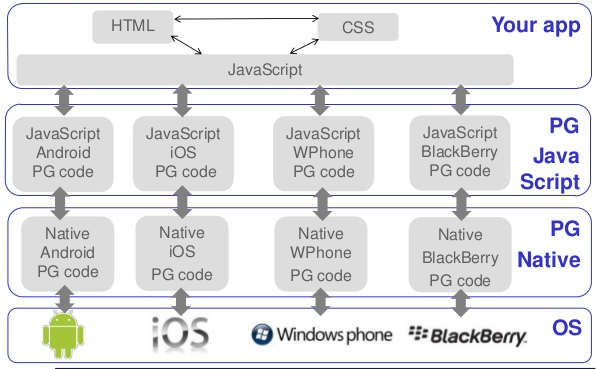
\includegraphics{Gambar/phonegap-architecture}
}
\caption[Arsitektur Phonegap]{Arsitektur Phonegap} 
\label{fig:arsitektur_phonegap}
\end{figure}

\section{Hadoop and \textit{Ecosystem}}
\label{sec:hadoopandecosystem}

\subsection{Hadoop}
\label{subsec:hadoop}

Hadoop merupakan sebuah \textit{platform} yang menyediakan pemyimpanan data terdistribusi dan kemampuan komputasi yang merupakan \textit{distributed master-slave architeture} yang terdiri dari Hadoop Distributed File System (HDFS)\ref{subsec:hdfs} untuk penyimpanan data dan MapReduce \ref{subsec:mapreduce} untuk melakukan komputasi dapat dilihat pada gambar \ref{fig:arsitektur_hadoop}\cite{holmes2012hadoop}.

\begin{figure}
\centering
\resizebox{\textwidth}{!}{
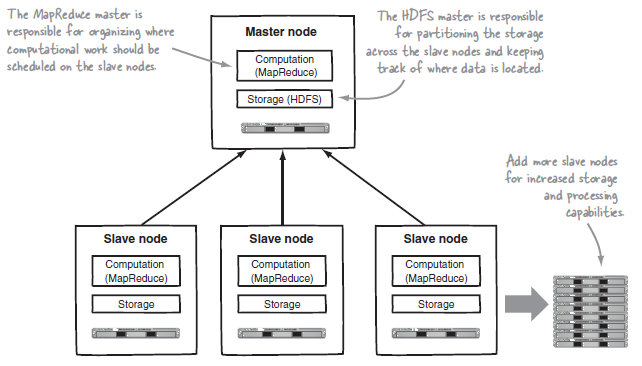
\includegraphics{Gambar/high-level-hadoop-architecture}
}
\caption[Arsitektur Hadoop]{Arsitektur Hadoop} 
\label{fig:arsitektur_hadoop}
\end{figure}

\subsection{HDFS}
\label{subsec:hdfs}

HDFS adalah komponen penyimpanan data dari Hadoop yang merupakan distem penyimpanan data terdistribusi. Arsitektur HDFS dapat dilihat pada Gambar\ref{fig:arsitektur_hdfs}

\begin{figure}
\centering
\resizebox{\textwidth}{!}{
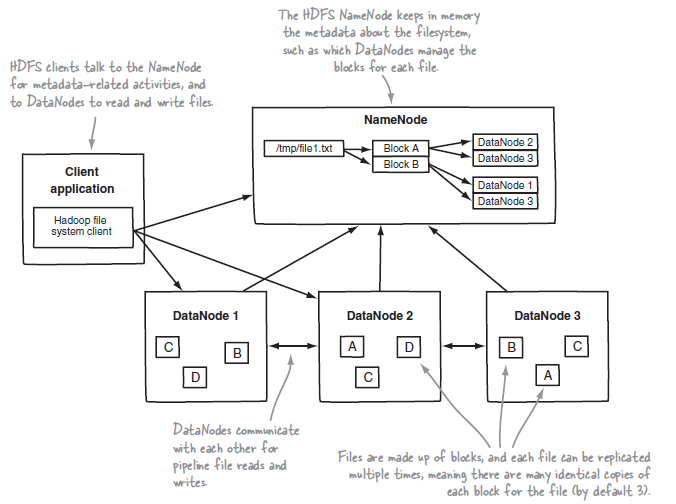
\includegraphics{Gambar/arsitektur-hdfs}
}
\caption[Arsitektur HDFS]{Arsitektur HDFS} 
\label{fig:arsitektur_hdfs}
\end{figure}

\subsection{MapReduce}
\label{subsec:mapreduce}

MapReduce merupakan \textit{batch-based}, komputasi terdistribusi \textit{framework} yang memungkinkan komputasi paralel terhadap data yang cukup besar. MapReduce menyederhanakan pemrosesan paralel oleh abstraksi kerja yang komplek. Dengan abstraksi ini, MapReduce memungkinkan para \textit{programmer} untuk berfokus pada kebutuhan bisnis dibandingkan memikirkan sistem distrubusinya.

\subsection{HBase}
\label{subsec:hbase}

HBase merupakan \textit{real-time, column-oriented} basis data yang dapat diintergrasi kedalam HDFS melalu MapReduce.

\subsection{Trafodion}
\label{subsec:trafodian}

Trafodion merupakan \textit{open source project} yang disponsor oleh HP, diinkubasi di HP Labs dan HP-IT yang digunakan untuk mengembangkan SQL-on-Hadoop berskala \textit{enterprise} terhadap data yang besar\footnote{https://wiki.trafodion.org/wiki/index.php/Main\_Page}. 

\section{Webservice and RESTful}
\label{sec:webserviceansrestful}

Pada sub-bab ini akan dibahas mengenai Webservice dan RESTful.

\subsection{Webservice}
\label{subsec:webservice}

Webservice merupakan suatu sistem yang menyediakan fungsi-fungsi dari suatu perangkat lunak diatas internet melalui \textit{web}. 

\subsection{RESTful}
\label{subsec:restful}

\textit{Representational State Transfer}(REST) merupakan gaya arsitektur suatu perangkat lunak yang terdiri dari pedoman dan pratek terbaik  untuk membuat suatu \textit{webservice}\ref{subsec:webservice} yang \textit{scalable}\footnote{Fielding, R. T.; Taylor, R. N. (2000). "Principled design of the modern Web architecture". pp. 407\-416. doi:10.1145/337180.337228}

\section{Google Open Authentication (OAuth)}
\label{sec:googleopenauthentication}

Pada sub-bab ini akan dibahas mengenai OAuth dan Google Oauth.

\subsection{Open Authentication (OAuth)}
\label{subsec:oauth}

OAuth merupakan standar terbuka untuk autentikasi. Oauth menyediakan akases yang aman kepada klien untuk mengakses \textit{server}. Hal ini mejadikan \textit{server} dapat diakses oleh \textit{third-party}. Disain OAuth diatas HTTP. Prinsip OAuth pada dasarnya menyediakan akses token kepada klien/pengguna akhir sehingga dapat digunakan untuk bertransaksi dengan \textit{server}\footnote{http://tools.ietf.org/html/rfc6749}.

\subsection{Google \textit{OAuth}}
\label{subsec:googleip}

Google OAuth merupakan protokol OAuth yang digunakan oleh google untuk memberikan akses kepada \textit{third-party} untuk mengakses API mereka. Skema pengakses Google OAuth dapat dilihat pada Gambar~\ref{fig:google_oauth}.

\begin{figure}
\centering
\resizebox{\textwidth}{!}{
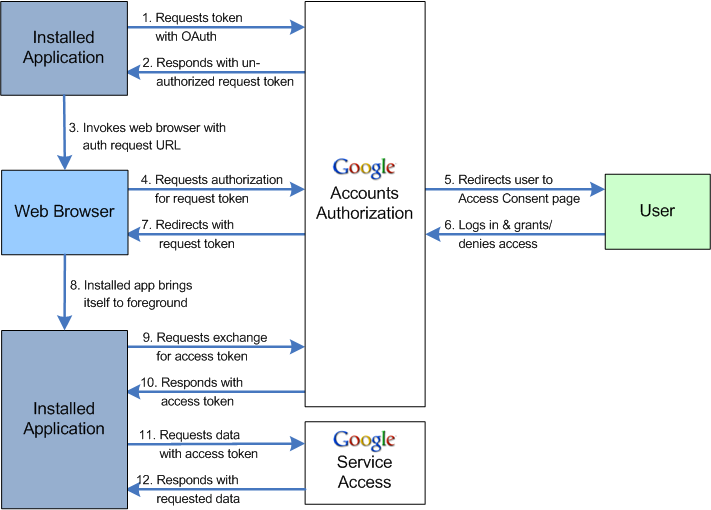
\includegraphics{Gambar/google-oauth}
}
\caption[Google OAuth]{Google OAuth} 
\label{fig:google_oauth}
\end{figure}